% !TEX root = ../Thesis.tex
% !TEX output_directory = ../
\chapter{Το Σύνολο Δεδομένων Και Οι Τροποποιήσεις Στις Οποίες Προβήκαμε} \label{dataset}


\section{MPII Cooking Activities Dataset \cite{rohrbach_2012}}
Το σύνολο δεδομένων MPII Cooking Activities Dataset περιλαμβάνει 44 βίντεο μαγειρικής στα οποία εμφανίζονται 65 κατηγορίες δράσεων. Από αυτές, οι 64 αφορούν δράσεις σχετικές με τη μαγειρική άμεσα (π.χ. πλύσιμο και κοπή φρούτων) ή έμμεσα (π.χ. εξαγωγή υλικού από το ψυγείο). Μία επιπλέον κατηγορία είναι η κλάση δράσεων υποβάθρου (background activity), που περιλαμβάνει τα τμήματα του βίντεο στα οποία δε συμβαίνει κάποια δράση ενδιαφέροντος από τις υπόλοιπες 64. Ο πίνακας \ref{tab:DataActions} περιέχει το σύνολο των δράσεων οι οποίες εμφανίζονται στο σύνολο MPII Cooking Activities Dataset. Από αυτές τις κατηγορίες, κρίνουμε ότι οι δράσεις put on cutting-board, read και smell ελάχιστα ενδιαφέρουν τη ροή της δράσης, οπότε κατατάσσονται στις δράσεις υποβάθρου. Ταυτόχρονα, η δράση wash hands δεν αφορά τη ροή και δεν διακρίνεται αρκετά από την δράση wash objects. Οπότε συνενώνουμε τις δύο κατηγορίες σε μία, με ενιαίο τίτλο wash objects. Επομένως, χρησιμοποιούμε τις 61 από τις 65 δράσεις.

\begin{table}
	\begin{tabular}{|p{13.5cm}|}
		\hline
		Actions in MPII Cooking Activities Dataset \\ \hline
		Background activity, change temperature, cut apart, cut dice, cut in, cut off ends, cut out inside, cut slices, cut stripes, dry, fill water from tap, grate, lid: put on, lid: remove, mix, move from X to Y, open egg, open tin, open/close cupboard, open/close drawer, open/close fridge, open/close oven, package X, peel, plug in/out, pour, pull out, puree, put in bowl, put in pan/pot, put on bread/dough, put on cutting-board, put on plate, read, remove from package, rip open, scratch off, screw close, screw open, shake, smell, spice, spread, squeeze, stamp, stir, strew, take \& put in cupboard, take \& put in drawer, take \& put in fridge, take \& put in oven, take \& put in spice holder, take ingredient apart, take out from cupboard, take out from drawer, take out from fridge, take out from oven, take out from spice holder, taste, throw in garbage, unroll dough, wash hands, wash objects, whisk, wipe clean. \\
		\hline
	\end{tabular}
	\caption{Οι 65 δράσεις του συνόλου δεδομένων MPII Cooking Activities Dataset. Στα πειράματά μας, οι δράσεις put on cutting-board, read και smell ενσωματώνονται στην κατηγορία background activity και η δράση wash hands συνενώνεται με τη δράση wash hands.}
	\label{tab:DataActions}
\end{table}



\par Τα 44 βίντεο ακολουθούν μια σύμβαση ονομασίας τύπου sSS-dDD, με τα SS και DD να αποτελούν διψήφιους αριθμούς που υποδεικνύουν το υποκείμενο, δράστη του βίντεο που εκτελεί τη συνταγή, (s από το subject) και το πιάτο-συνταγή (d από το dish) αντίστοιχα. Για παράδειγμα, έγκυρη ονομασία είναι η s19-d07, που υποδηλώνει ότι ο δράστης 19 εκτελεί τη συνταγή 7. Στο σύνολο των 44 βίντεο, εμφανίζονται διάφοροι συνδυασμοί υποκειμένων από το 8 ως το 20 και πιάτων από το 1 ως το 14. Είναι φανερό ότι το σύνολο δεδομένων περιέχει ένα υποσύνολο όλων των πιθανών συνδυασμών δραστών και συνταγών. Τα βίντεο που περιέχονται φαίνονται στον πίνακα \ref{tab:DataVideos}. Από αυτά, επιλέχθηκαν ως βίντεο εκπαίδευσης όσα αφορούν τους δράστες 11 ως 15. Επειδή κάποιες κατηγορίες δεν περιέχονταν στα βίντεο αυτά, προσθέσαμε στα βίντεο εκπαίδευσης επιπλέον τα s08-d02 και s10-d10. Όλα τα βίντεο είναι πυκνά δειγματοληπτημένα στα 29.4 frames ανά δευτερόλεπτο. Η συνολική διάρκεια των βίντεο, εκπαίδευσης και ελέγχου είναι περίπου 8 ώρες, επομένως ο αριθμός των συνολικών frames ξεπερνά τις 800000.

\begin{table}
    \begin{tabular}{|p{13.5cm}|}
    \hline
    Videos in MPII Cooking Activities Dataset \\ \hline
    s08-d02, s08-d04, s08-d11, s08-d14, s10-d02, s10-d10, s10-d11, s11-d01, s11-d06, s11-d11, s11-d12, s11-d13, s11-d14, s12-d05, s12-d07, s12-d09, s12-d10, s12-d14, s13-d08, s13-d09, s13-d11, s13-d12, s13-d13, s14-d08, s14-d09, s14-d11, s15-d03, s15-d07, s15-d14, s16-d01, s16-d06, s16-d09, s16-d11, s17-d02, s17-d05, s17-d13, s18-d11, s19-d01, s19-d06, s19-d07, s19-d09, s19-d10, s19-d12, s20-d07. \\
    \hline
    \end{tabular}
	\caption{Τα 44 βίντεο του συνόλου δεδομένων MPII Cooking Activities Dataset. Από αυτά, χρησιμοποιούμε για εκπαίδευση όσα αφορούν τους δράστες 11 ως 15 και τα s08-d02 και s10-d10.}
	\label{tab:DataVideos}
\end{table}


\par Στις επισημειώσεις των βίντεο παρέχονται τα όρια (πρώτο και τελευταίο frame) κάθε δράσης, ο κωδικός της δράσης (ένας ακέραιος από 1 ως 65) και το όνομα της δράσης. Επομένως τα βίντεο έχουν επισημειώσεις ιδανικές για αξιολόγηση αναγνώρισης και κατάτμησης δράσεων. Καθώς η αυθεντική εργασία \cite{rohrbach_2012} που εισήγαγε το σύνολο δεδομένων αξιοποιεί τη μέθοδο Πυκνών Τροχιών \cite{wang_2011} για την αναπαράσταση των βίντεο, συνδυαζόμενη με χαρακτηριστικά πόζας \cite{andriluka_2009}, οι ερευνητές παραθέτουν τα υπολογισμένα χαρακτηριστικά (HOG, HOF, MBH, Περιγραφητής Τροχιάς, Μοντέλα Σώματος, FFT) για το σύνολο των βίντεο. Η σημασία και η φύση των χαρακτηριστικών αυτών είναι θέμα του κεφαλαίου 3. Τα χαρακτηριστικά παρέχονται σε κωδικοποιημένη μορφή με τη μέθοδο k-μέσων και k=4000, ενώ για ευκολία χειρισμού παρέχονται τα ολοκληρωτικά ιστογράμματα χαρακτηριστικών. Ο ενδιαφερόμενος μπορεί να βρει περισσότερες πληροφορίες και υλικό για το σύνολο MPII Cooking Activities Dataset στην τοποθεσία \url{https://www.mpi-inf.mpg.de/departments/computer-vision-and-multimodal-computing/research/human-activity-recognition/mpii-cooking-activities-dataset/}.


\section{MPII Cooking 2 Dataset \cite{rohrbach_2015}}
Το σύνολο MPII Cooking 2 Dataset αποτελεί επέκταση του MPII Cooking Activities Dataset και περιλαμβάνει 273 βίντεο μαγειρικής με περισσότερες δράσεις και επισημειώσεις. Η σύμβαση για την ονομασία των βίντεο παραμένει. Δεν θα αναφερθούμε με λεπτομέρεια στα βίντεο και τις δράσεις του συνόλου καθώς δεν χρησιμοποιούνται αυτά καθαυτά τα δεδομένα στη δική μας εργασία. Θα εστιάσουμε στις επιπλέον επισημειώσεις τις οποίες αξιοποιούμε, τονίζοντας πρώτα ότι οι δράσεις και τα βίντεο του MPII Cooking Activities Dataset είναι υποσύνολα των δράσεων και των βίντεο του MPII Cooking 2 Dataset.

\par Το σύνολο MPII Cooking 2 Dataset περιέχει επισημειώσεις αρκετά πλουσιότερες αυτών του MPII Cooking Activities Dataset. Αρχικά, παρέχονται επισημειώσεις δράσεων για κάθε βίντεο στη μορφή: έναρξη (σε χρόνο και frames) και λήξη δράσης, είδος δράσης, δράστης και σύνολο αντικειμένων που πλαισιώνουν τη δράση. Τα αντικείμενα αυτά χωρίζονται επιπλέον σε εργαλεία και υλικά, αλλά η διάκριση αυτή δεν αφορά την εργασία μας. Με βάση τις επισημειώσεις αυτές, αποκτούμε έναν χρονικό χάρτη των αντικειμένων που εμφανίζονται στο βίντεο. Βέβαια υπογραμμίζουμε το ότι οι επισημειώσεις αυτές αφορούν τα αντικείμενα που χρησιμοποιούνται στην κάθε δράση και όχι αυτά που εμφανίζονται οπτικά στο βίντεο σε κάθε χρονική στιγμή. Τα αντικείμενα που εμφανίζονται κατατάσσονται σε 155 κατηγορίες, από τις οποίες μας ενδιαφέρουν μόνο οι 92, καθώς αυτές εμφανίζονται στα βίντεο του MPII Cooking Activities Dataset. Επιπλέον, στις 92 κατηγορίες δεν περιλαμβάνονται συγκεκριμένα ουσιαστικά όπως χέρι και πάγκος, καθώς δεν δίνουν ιδιαίτερη πληροφορία για τη δράση. Το σύνολο των ουσιαστικών που χρησιμοποιούνται στα πειράματά μας φαίνεται στον πίνακα \ref{tab:DataNouns}.

\begin{table}
    \begin{tabular}{|p{13.55cm}|}
    \hline
    Objects in MPII Cooking 2 Dataset \\ \hline
    apple, baking tray, blender, bottle, bowl, box grater, bread, bread knife, butter, carrot, cheese, chefs knife, chocolate, colander, corn, cucumber, cup, cupboard, dough, drawer, egg, eggshell, electricity column, electricity plug, flat grater, fridge, front peeler, frying pan, garbage, garlic clove, glass, ham, hot chocolate powder bag, jar, kiwi, knife, kohlrabi, ladle, lemon, lid, masher, measuring pitcher, milk, mushroom, oil, onion, orange, oven, paper, paper box, peach, pear, peel, pepper, pineapple, plastic bag, platic bottle, plastic box, plastic paper bag, plate, plum, pot, potato, puree, salad, salami, salt, seed, side peeler, sink, soup, spatula, spice, spice holder, spice shaker, sponge, sponge cloth, spoon, squeezer, stone, stove, tap, teaspoon, tin, tin opener, tomato, towel, water, wire whisk, wrapping paper, yolk, zucchini. \\
    \hline
    \end{tabular}
	\caption{Οι 92 κατηγορίες αντικειμένων που εμφανίζονται στα βίντεο του συνόλου MPII Cooking Activities Dataset και που χρησιμοποιούμε στα πειράματά μας.}
	\label{tab:DataNouns}
\end{table}

\par Σε παλιότερη εργασίων των ερευνητών \cite{regneri_2013}, είχε σχεδιαστεί σύστημα αυτόματης εξαγωγής λεκτικών περιγραφών για τα βίντεο της πρώτης έκδοσης του MPII Cooking 2 Dataset. Για την εγκυρότητα αυτών των περιγραφών, είχε συλλεχθεί από τους ερευνητές ένα σύνολο ανθρώπινων περιγραφών για τις δράσεις και τα αντικείμενα των βίντεο. Οι επισημειώσεις του MPII Cooking 2 Dataset ενσωματώνουν τις περιγραφές αυτές, προβαίνοντας σε εξαγωγή από κοινού εμφανίσεων δράσεων και αντικειμένων. Μια απο κοινού εμφάνιση πραγματοποιείται όταν το ρήμα της δράσης και τα ουσιαστικά των αντικειμένων συνυπάρχουν στην ίδια πρόταση. Με βάση αυτές τις περιγραφές μπορούμε να εξάγουμε την πρότερη πιθανότητα εμφάνισης της δράσης $\alpha$ δεδομένης της εμφάνισης του αντικειμένου $object$, $P(\alpha|object)$. Η διαδικασία αυτή αναλύεται στο κεφάλαιο 6. Περισσότερες λεπτομέρειες και υλικό για το σύνολο MPII Cooking 2 Dataset μπορούν να βρεθούν στην τοποθεσία \url{https://www.mpi-inf.mpg.de/departments/computer-vision-and-multimodal-computing/research/human-activity-recognition/mpii-cooking-2-dataset/}.


\section{Επιπλέον Επισημειώσεις Στις Οποίες Προβήκαμε}
\subsection{Υπότιτλοι}
Για την αξιοποίηση της ομιλίας ως τρόπο έκφρασης επιπλέον πληροφορίας, προβαίνουμε σε ανάλυση υποτίτλων, ώστε να αποφύγουμε τα σφάλματα που θα εισήγαγε ένα σύστημα αυτόματης αναγνώρισης λόγου, καθώς αυτό ξεφεύγει από τον σκοπό αυτής της εργασίας. Επειδή δεν υπάρχουν υπότιτλοι για το MPII Cooking Activities Dataset, δημιουργήσαμε εμείς. Σε ένα σύνολο επισημειωτών δόθηκε το βίντεο και οι επισημειώσεις δράσεων και αντικειμένων από το MPII Cooking 2 Dataset. Επιβάλλαμε τον περιορισμό της χρήσης των ονομάτων των αντικειμένων απευθείας και όχι συνωνύμων τους, καθώς στη χρήση των υποτίτλων αναζητούμε μόνο τα ονόματα των αντικειμένων όπως αυτά παρέχονται από το MPII Cooking 2 Dataset. Όσον αφορά τους χρόνους ενός επιλόγου, επιβάλλαμε να εκτείνονται εντός της διάρκειας της δράσης και το χρονικό τους μήκος να περιορίζεται κάτω από τα 15 δευτερόλεπτα, ανάλογα πάντα με το μέγεθος του διαλόγου σε λέξεις. Προσπαθήσαμε να διατηρήσουμε τη φυσικότητα των υποτίτλων και ταυτόχρονα να διευκολύνουμε την ανίχνευση αντικειμένων μέσω αυτών. Στον πίνακα \ref{tab:DataSubtitles} φαίνεται ένα παράδειγμα τμήματος των υποτίτλων για το βίντεο s08-d04.

\begin{table}
    \begin{tabular}{ | l | l | l |}
    \hline
    Start Time & End Time & Subtitle \\ \hline
    714.7200 & 722.7210 & Pour enough oil to fill the bottom of your frying-pan. \\ \hline
	723.0950 & 726.9380 & Spread it uniformly. \\ \hline
	728.4170 & 730.6840 & Ok, turn on the stove in this point. \\ \hline
	730.7240 & 734.8660 & Choose a high temperature for start. \\
    \hline
    \end{tabular}
	\caption{Παράδειγμα υποτίτλων για το βίντεο s08-d04. Όλοι οι χρόνοι αναφέρονται σε δευτερόλεπτα από την αρχή του βίντεο.}
	\label{tab:DataSubtitles}
\end{table}


\subsection{Επισημειώσεις Αντικειμένων}
Το σύνολο MPII Cooking 2 Dataset περιέχει επισημειώσεις για τα αντικείμενα που χρησιμοποιούνται ανά δράση. Ωστόσο, οπτική επισημείωση, για τη θέση δηλαδή του χρησιμοποιούμενου αντικειμένου στα frames, δεν υπάρχει. Προκειμένου να εντοπίσουμε οπτικά τα αντικείμενα στα frames του βίντεο, είναι φανερό ότι πρέπει να έχουμε δεδομένα για την εμφάνιση τους. Καθώς η μεταβλητότητα των αντικειμένων είναι εξαιρετικά μεγάλη (όπως αναλύουμε στο κεφάλαιο 4), δημιουργούμε μοντέλα αντικειμένων για κάθε βίντεο ξεχωριστά. Η δημιουργία επισημειώσεων έγινε σε δύο στάδια, τα οποία εξυπηρετούν διαφορετικούς σκοπούς.

\par Σε πρώτη φάση, δειγματοληπτούμε το βίντεο με περίοδο 100 frames και σε κάθε ένα σημειώνουμε τα αντικείμενα που εμφανίζονται. Η διαδικασία αυτή γίνεται με τη λειτουργία trainingImageLabeler του λογισμικού MATLAB. Με το λογισμικό αυτό, είναι εύκολο να δημιουργηθεί ένα ορθογώνιο που περιλαμβάνει την περιοχή ενδιαφέροντος. Ο χρήστης εισάγει τα ορθογώνια και τις ετικέτες και το πρόγραμμα εξάγει τις χωρικές συντεταγμένες πάνω στο frame. Ένα παράδειγμα φαίνεται στην παρακάτω εικόνα:

\begin{figure}[H]
  \centering
  \noindent\makebox[\textwidth]{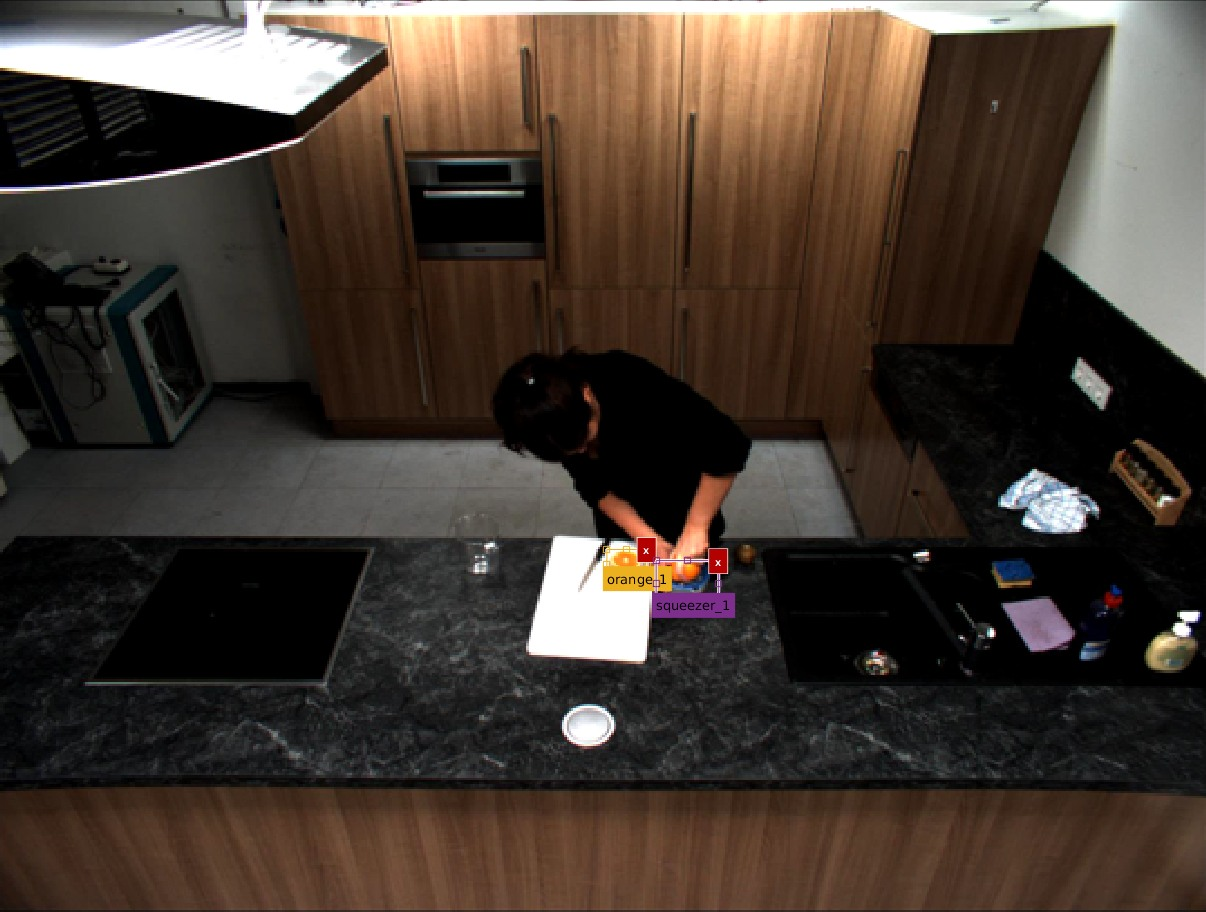
\includegraphics[scale=0.25]{{Images/AppMatlab}.jpg}}
  \caption{Παράδειγμα δημιουργίας επισημειώσεων με το λογισμικό trainingImageLabeler του MATLAB. Εισάγουμε τα ορθογώνια και την ετικέτα και το λογισμικό εξάγει τις συντεταγμένες. Η χρήση του πακέτου αυτου διευκολύνει τη μαζική δημιουργία θετικών δειγμάτων εκπαίδευσης για ανιχνευτές αντικειμένων.}
  \label{fig:AppMatlab}
\end{figure}

\par Προσπαθούμε να σημειώνουμε τα αντικείμενα τα οποία μένουν σχετικά σταθερά εμφανισιακά σε αρκετά frames κι έτσι μπορούν να εντοπιστούν από έναν ανιχνευτή όπως ο \cite{viola_2001}. Έτσι, επιλέγουμε να δημιουργούμε αντιπροσώπους κλάσεων με τμήματα αντικειμένων που παραμένουν σταθερά και εντός της περιοχής ενδιαφέροντος. Για παράδειγμα στην παραπάνω εικόνα, το πορτοκάλι που κείται δίπλα στον στίφτη μπορεί να εντοπιστεί. Εν τούτοις δεν είναι αυτό το πορτοκάλι που βρίσκεται εν χρήση αλλά ένα τμήμα του που μένει ακίνητο. Παρόμοια στρατηγική ακολουθείται για τις υπόλοιπες κατηγορίες αντικειμένων. Ως ένα ακόμα παράδειγμα, τα έπιπλα αναπαρίστανται με την εμφάνιση ή μη του τμήματός τους που φαίνεται όταν αυτά χρησιμοποιούνται (ανοίγουν). Στην παρακάτω εικόνα φαίνεται ένα τέτοιο παράδειγμα για την περίπτωση του ψυγείου.

\begin{figure}[H]
  \centering
  \noindent\makebox[\textwidth]{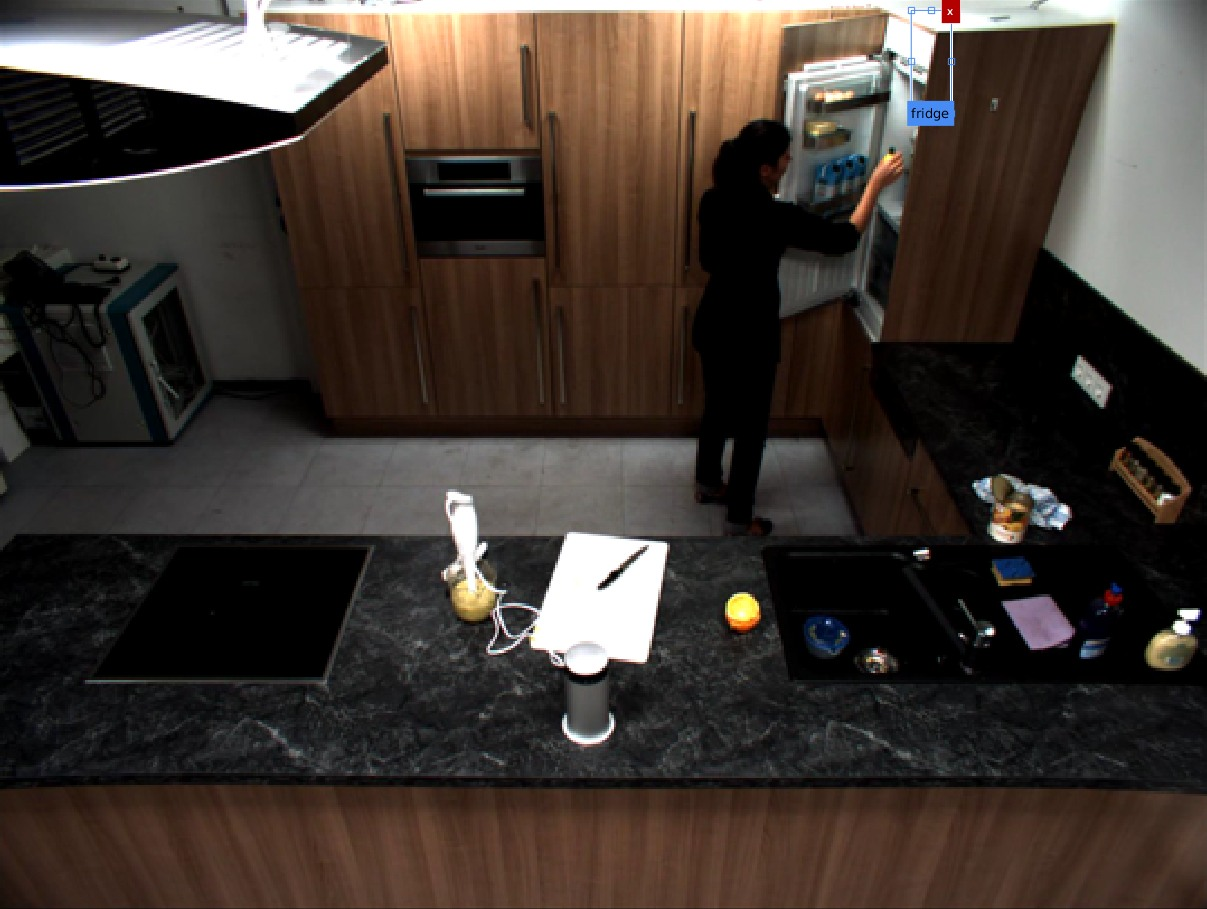
\includegraphics[scale=0.25]{{Images/AppFridge}.jpg}}
  \caption{Παράδειγμα αναπαράστασης σταθερού αντικειμένου με το τμήμα του το οποίο εμφανίζεται μόνο όταν το αντικείμενο χρησιμοποιείται. Έτσι, εξασφαλίζεται ότι το αντικείμενο θα εντοπίζεται μόνο σε περιπτώσεις ενδιαφέροντος και όχι σε όλη τη διάρκεια του βίντεο.}
  \label{fig:AppFridge}
\end{figure}

\par Οι επισημειώσεις αυτές λειτουργούν ως θετικά δείγματα για εκπαίδευση ενός ανιχνευτή αντικειμένων. Λόγω της υψηλής μεταβλητότητας, επιλέξαμε τη χρήση Ταιριάσματος Προτύπων (Template Matching) ως ανιχνευτή αντικειμένων κι έτσι απαιτούνταν να συλλέξουμε πρότυπα. Έχοντας λοιπόν τις πλήρεις επισημειώσεις μέσω του trainingImageLabeler, επιλέξαμε αυτές που εμφανίζοταν συχνά και για μεγάλη χρονική διάρκεια ως αντιπροσώπους κλάσεων αντικειμένων. Πρακτικά, συρρικνώνουμε τα θετικά δείγματα έτσι ώστε να ελαχιστοποιείται η απώλεια που αυτό συνεπάγεται στην μεταβλητότητα και στον ικανοποιητικό εντοπισμό. Στο κεφάλαιο 4 αναλύουμε περισσότερα για τη μέθοδο εντοπισμού των αντικειμένων.


\subsection{Επισημειώσεις Χεριών}
Στο κεφάλαιο 5 δείχνουμε τον εντοπισμό χεριών και την εξαγωγή του τύπου λαβής (grasping type). Στο κεφάλαιο 6, τα αποτελέσματα φαίνονται να υποβοηθούνται από αυτή την πληροφορία. Εν τούτοις, σύνολο δεδομένων δεν υπήρχε ούτε σχετικά με τον εντοπισμό χεριών, ούτε σχετικά με την εξαγωγή τύπου λαβής, που να σχετίζονται άμεσα με το MPII Cooking Activities Dataset. Επομένως, έπρεπε να δημιουργήσουμε, με βάση τις διαθέσιμες πληροφορίες, μια βάση για τον εντοπισμό χεριών αρχικά.

\par Παρότι υπάρχουν διάφοροι επιτυχείς αλγόριθμοι και σύνολα δεδομένων \cite{mittal_2011} για ανίχνευση χεριών, ακολουθούμε την πρόταση του \cite{rohrbach_2015} και επανεκπαιδεύουμε έναν ανιχνευτή χεριών με εικόνες που επιλέγονται αραιά από το σύνολο δεδομένων MPII Cooking Activities Dataset. Για τις εικόνες εκπαίδευσης, συνενώνουμε τα σύνολα δεδομένων πόζας \cite{amin_2013} και \cite{rohrbach_2012}. Οι επισημειώσεις των συνόλων αυτών είναι σύνολα σημείων που αναπαριστούν τις θέσεις διαφόρων συνδέσμων του άνω τμήματος του σώματος. Δύο από αυτές τις επισημειώσεις αφορούν το αριστερό και το δεξί χέρι. Ωστόσο, οι επισημειώσεις δεν εξασφαλίζουν ότι τα χέρια φαίνονται στην εικόνα, παρά μόνο δείχνουν το πού αυτά βρίσκονται. Δύο παραδείγματα φαίνονται στην εικόνα \ref{fig:AppHands}, όπου στην δεύτερη περίπτωση βλέπουμε μια φυσιολογική απεικόνιση των χεριών, ενώ στην πρώτη, βλέπουμε σημεία να απεικονίζουν τη θέση των χεριών πίσω από το υπόλοιπο σώμα του ανθρώπου. Οπότε σε πρώτη φάση, σκανάραμε το σύνολο αυτών των εικόνων και κρατήσαμε μόνο αυτές για τις οποίες φαίνονταν τα χέρια. Για εικόνες που φαινόταν μόνο το ένα χέρι, κρατήσαμε ετικέτες ώστε στη φάση εξαγωγής θετικών δειγμάτων να λάβουμε την εικόνα μόνο του χεριού που εμφανίζεται. Σε δεύτερη φάση, εξαγάγαμε ορθογώνια που περιέκλειαν τα χέρια. Πειραματικά διαπιστώσαμε ότι κουτιά σταθερού μεγέθους $31 \times 31$ είναι επαρκή για τη συμπερίληψη του χεριού ανεξαρτήτως της απόστασης από την κάμερα. Τέλος, λάβαμε αρνητικά δείγματα κυλώντας ένα παράθυρο με βήμα 5 σε οριζόντιο και κάθετο άξονα ανά εικόνα και λαμβάνοντας έτσι δύο τυχαία δείγματα μη χεριών από κάθε εικόνα. Αν 6 εικόνες, χρησιμοποιήσαμε το άνω τμήμα του κεφαλιού ως επιπλέον αρνητικό δείγμα, ενώ επίσης ανά 6, αλλά με άλλη αρχή μέτρησης, χρησιμοποιήσαμε το κάτω μέρος του κεφαλιού για αρνητικό δείγμα. Η διαδικασία που ακολουθεί περιγράφεται στο κεφάλαιο 5.

\par Η έλλειψη επισημειώσεων για τον τύπο λαβής μας ανάγκασε να χρησιμοποιήσουμε μη επιβλεπόμενη μάθησης, όπως περιγράφεται στο κεφάλαιο 5. Επομένως, δημιουργούμε ένα σύνολο δεδομένων τύπων λαβής με αυτόματο τρόπο, λύνοντας το πρόβλημα απουσίας επισημειώσεων και δεν προβαίνουμε σε επιπλέον διαδικασίες επισημειώσεων.

\begin{figure}
  \centering
  \noindent\makebox[\textwidth]{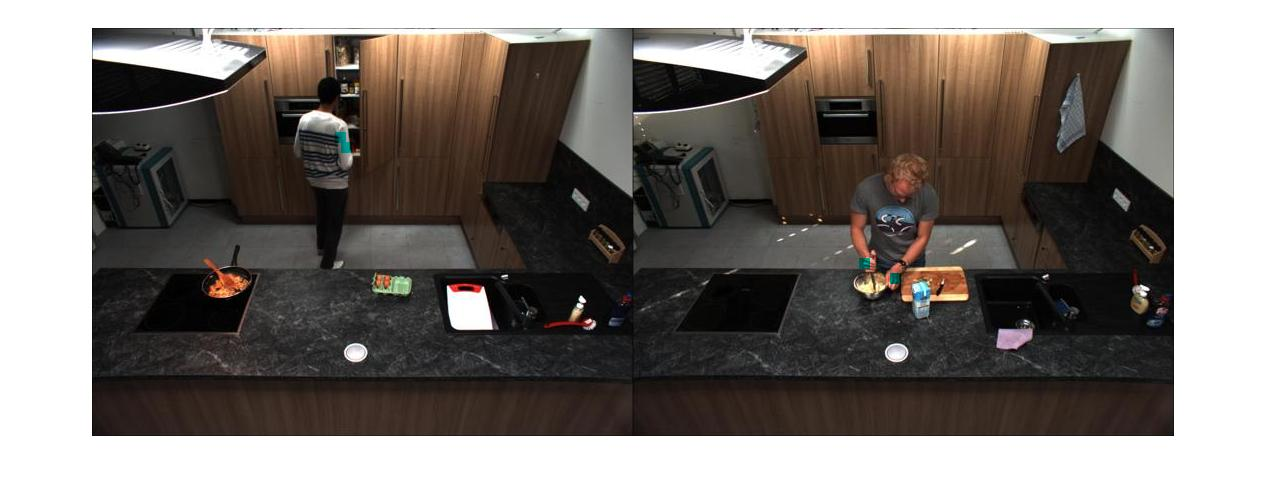
\includegraphics[scale=0.35]{{Images/AppHands}.jpg}}
  \caption{Παραδείγματα επισημειώσεων πόζας. Με μπλε απεικονίζονται τα σημεία που χαρακτηρίζονται ως χέρια μέσω των επισημειώσεων πόζας. Δείχνουμε τις περιοχες ως τετράγωνα $10 \times 10$ γύρω από τα σημεία επισημείωσης για να είναι εμφανείς οπτικά στον αναγνώστη. Βλέπουμε ότι ενώ στη δεξιά εικόνα οι επισημειώσεις ταυτίζονται με τη θέση των χεριών, τα οποία είναι εμφανή οπτικά, στην εικόνα αριστερά οι επισημειώσεις δείχνουν τη θέση που βρίσκεται το χέρι πίσω από το σώμα του ανθρώπου. Είναι φανερό ότι εικόνες σαν την αριστερή δεν μπορούν να χρησιμεύσουν σαν θετικά δείγματα για έναν ανιχνευτή χεριών και έτσι αποκλείονται από τα θετικά δεδομένα εκπαίδευσης και χρησιμοποιούντι μόνο για την εξαγωγή αρνητικών παραδειγμάτων.}
  \label{fig:AppHands}
\end{figure}



